\begin{frame}{What is Browser Fingerprinting}
  Browser Fingerprinting is a method that allows websites and online services to \textbf{collect} and \textbf{analyze} specific data about a user's device resulting in a \textbf{unique fingerprint} of it
  \begin{figure}
    \centering
    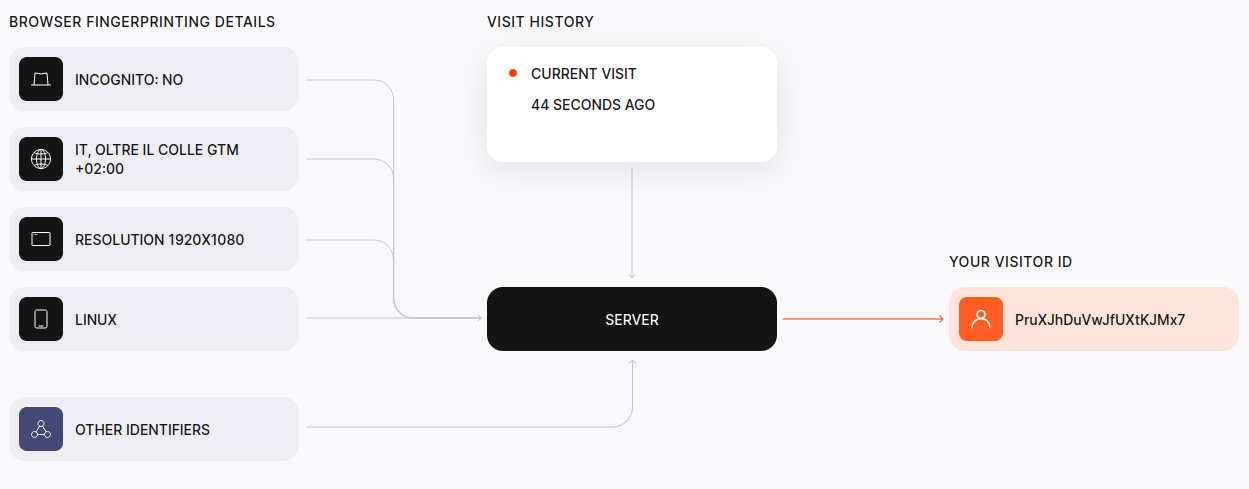
\includegraphics[width=\linewidth]{images/fingerprint.png}
  \end{figure}
\end{frame}

\begin{frame}{Collected data}
  \begin{itemize}
    \item \textbf{Browser info:} type, version, language, plugins, settings, \dots
          \vspace{1cm}
    \item \textbf{Device info:} OS, GPU, screen size, fonts, battery info, \dots
          \vspace{1cm}
    \item \textbf{Network and Session info:} public IP, local IP, VPN, timezone, supported protocols, \dots
  \end{itemize}
\end{frame}

\begin{frame}{Browser Fingerprinting properties: uniqueness}
  \begin{itemize}
    \item highly improbable for two users to have identical fingerprints
    \item \textbf{uniqueness can be so specific} that only one in several hundred thousand users might share the same fingerprint
  \end{itemize}
  \begin{figure}
    \centering
    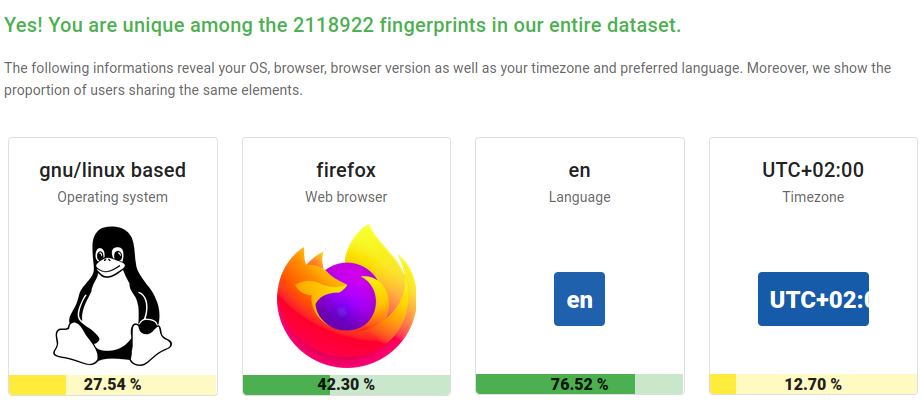
\includegraphics[width=\linewidth]{images/uniqueness.png}
  \end{figure}
\end{frame}

\begin{frame}{Browser Fingerprinting properties: stateless}
  \vspace{-0.5cm}
  Still works even if users:
  \begin{itemize}
    \item disable cookies
    \item change IP
    \item use privacy-focused browsing modes
  \end{itemize}
  \smallskip
  This method is stateless, not relying on stored data in the browser, and hence, it leaves no obvious trace.

  \begin{figure}
    \centering
    \begin{subfigure}{0.45\textwidth}
      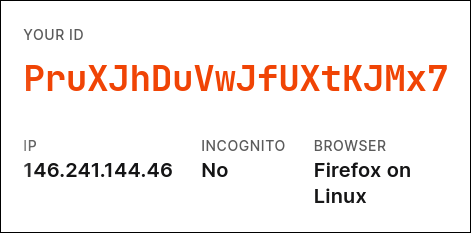
\includegraphics[width=\linewidth]{images/fingerprint-ip-1.png}
    \end{subfigure}
    \begin{subfigure}{0.45\textwidth}
      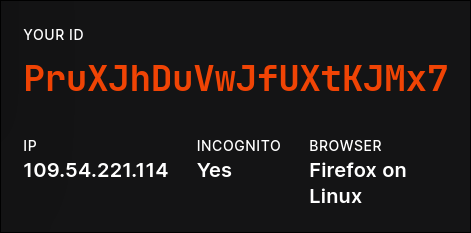
\includegraphics[width=\linewidth]{images/fingerprint-ip-2.png}
    \end{subfigure}
  \end{figure}
\end{frame}